\chapter{Реализация}
\label{chapter_implementation}

\section{Введение}
\label{sect_impl_introduction}

Реальные программы пользуются всеми возможностями языка Си, не все из которых были рассмотрены в теории.
Например, описанная теория не предполагает использования указателей и адресной арифметики.
Поэтому реализация рассмотренных анализов может некоторым образом отличаться от теоретического описания.
В разделе~\ref{sect_impl_overview} описаны реализации всех используемых анализов.

При переходе от теории к практике становится важным уделять большее внимание эффективности применяемых алгоритмов.
В разделе~\ref{sect_impl_storage} будут описаны оптимизации теоретически разработанных алгоритмов, которые позволяют применять их для реальных программных систем. 

Первая такая оптимизация касается хранения достижимых состояний. В теории для определения состояния гонки необходимо было для каждой пары достигнутых состояний проверить наличие обращения к одинаковой разделяемой памяти.
Такой простой алгоритм был совершенно не эффективен. Количество различных состояний может превышать десять миллионов.
Поэтому необходимы очень эффективные алгоритмы хранения и поиска пары состояний образующих состояние гонки. 

Процесс уточнения построенной абстракции может занимать достаточно много времени даже при решении задачи достижимости.
При поиске состояний гонки может быть необходимо уточнить абстракцию сразу для нескольких обнаруженных состояний гонки.
Уточнение абстракции последовательно становится очень неэффективным. В подразделе~\ref{sect_impl_refinement} описан процесс уточнения абстракции и применяемые оптимизации.

Важной задачей, на которую многие академические инструменты не обращают внимания, является понятное и наглядное представление результатов верификации.
Это особенно важно для описания ошибок, связанных с параллельным выполнением нескольких потоков, так как при этом не достаточно указать только строку или переменную, в которой возможно наличие ошибки.
Необходимо представить полную трассу выполнения потоков, выделив некоторые важные события, например, создание потоков, захват примитивов синхронизации и одновременные доступы к разделяемой памяти. В подразделе~\ref{sect_impl_visualization} будут описан алгоритм печати трассы.

\section{Устройство инфраструктуры CPAchecker}
\label{sect_impl_cpachecker}

CEGAR

\section{Реализация инструмента}
\label{sect_impl_overview}

\subsection{Анализ с раздельным анализом потоков}
\label{subsect_impl_tm}

\subsection{Анализ абстракций по блокам}
\label{subsect_impl_bam}

В процессе анализа используется оптимизация, использующая абстрактные блоки (англ. Block Abstraction Memoization, BAM). 
Эта оптимизация позволяется переиспользовать результаты, полученные в процессе анализа.
Например, если функция уже была проанализирована, и та же самая функция вызывается второй раз, анализировать ее заново не обязательно, если контекст ее вызова тот же самый.
Абстрактными блоками, на границах которых производится кэширование результатов, могут быть как функции, так и тела циклов. 

Каждый анализ описывает специальный механизм выделения существенной части из своего абстрактного состояния. Это операция reduce. 
По смыслу - эта операция избавляет от контекста при входе в новый блок.
При входе анализом в новый абстрактный блок выполняется операция reduce. Полученное "уменьшенное" состояние ищется в кэше.
В случае, если результат уже присутствует к кэше, то есть анализ для данного состояния уже проводился ранее, выполняется операция expand, которая на основе полного исходного состояния и неполного результирующего состояния строит полное результирующее состояние. 
Если же фиксируется промах в кэше, это значит, что нужно провести анализ и сохранить его результат. 

Существующая оптимизация BAM была предназначена для анализа на достижимость некоторого состояния.
Основная проблема заключается в восстановлении пути, приводящего к ошибочному состоянию.
В исходном варианте оптимизации BAM состояние было только одно - ошибочное, соответственно, ошибка могла быть зафиксирована, если анализ обнаружил путь к этому конкретному состоянию.
В этот момент можно завершать анализ и восстанавливать ошибочный путь.
При поиске состояний гонки приходится сначала строить все достижимые состояния, а затем искать те пары, которые образуют состояние гонки.
В этом случае может возникнуть неопределенность при восстановлении пути, если одна из функций на стеке вызовов может быть вызвана из нескольких мест.
В исходном варианте оптимизации анализ останавливается при получении первого же пути к ошибочному состоянию, и если бы на этом пути некоторая функция могла бы вызываться из другого места, то анализ должен был бы вначале исследовать этот путь и обнаружить путь к ошибочному состоянию раньше.

Для решения этой проблемы был сделан переработан механизм восстановления пути. 
При визуаилизации результатов нет необходимости показывать все возможные пути к некоторому доступу к памяти, однако в процессе уточнения необходимо проверить все варианты.
Подробнее про процесс уточнения результатов будет рассказано в соответствующем разделе.

\subsection{Анализ примитивов синхронизации}
Анализ примитивов синхнонизации соответствует описанному в теоретической части LockCPA (раздел~\ref{sect_lock_analysis}).
Теоретически описанный LockCPA имеет ряд допущений:
\begin{itemize}
\item захватываемый объект (блокировка) должен быть явно указан в операторе $acquire$/$release$;
\item никакие другие операторы, кроме $acquire$/$release$, не работают с примитивами синхронизации;
\item отсутствие рекурсивного захвата блокировки;
\end{itemize}

\subsubsection{Указатели на объекты блокировок}
В реальных же программах блокировки часто передаются в функцию захвата или освобождения по указателям.
При этом указатели могут храниться в полях различных структур.
Это значительно усложняет задачу определения реального объекта блокировки, с помощью которого производится синхронизация.
Во многих статьях, которые задаются вопросом применения своих инструментов к реальному программному обеспечению, часто применяют анализ указателей для вычисления объектов, на которые могут указывать те указатели, которые используются при захвате блокировки.
Однако, как и всякий анализ указателей, такой подход имеет ряд недостатков, главными из которых являются его эффективность и точность.
Дело в том, что анализ указателей Андерсена (и его различные вариации) может применяться только если указатели должным образом инициализируются.
В случае же если инициализация указателя не была проведена, и этому указателю не была поставлена в соответствие некоторая память, такой анализ будет некорректным.
В нашем случае инициализация многих указателей может отсутствовать, так как не весь исходный код может доступен.

Все это приводит к тому, что определить точное соответствие указателей в общем случае становится невозможным.
Приходится делать некоторое разумное предположение о том, что захват блокировки и ее освобождение, скорее всего, будет производится одинаковым образом.
Например, если был использован указатель на объект при захвате, то он же будет использован и при освобождении.
А если при захвате использовался указатель на поле структуры, то и при освобождении будет передан указатель на поле с тем же именем и структуры того же типа.
Таким образом, становится возможно, в соответствии с теорией, по имени переменной, быть может указателю, явно идентифицировать тот объект, с которым производится работа.

\subsubsection{Неявные операции работы с примитивами синхронизации}
В пользовательских программах используется выделенный интерфейс для работы с примитивами синхронизации, который предоставляет операционная система.
В POSIX это функции pthread\_mutex\_lock/pthread\_mutex\_unlock. 
Однако, компоненты операционной системы внутри себя могут использовать различные примитивы синхронизации напрямую.
Например, проверять, включено ли планирование, которое также может выступать в роли особой (глобальной) блокировки.
При этом такая проверка может быть, как через специальный интерфейсный макрос/функции, например, $dispatchEnable()$, так и через явное обращение к переменной $dispatchEnable == 1$\footnote{Пример кода является вымышленным, совпадение с какой-либо известной операционной системой является случайным}.
Кроме того, отключение планирование (захват блокировки) может также проводиться с помощью интерфейсного макроса/функции $dispatchDisable()$ или напрямую $dispatchDisable = 1$.
Хотя явное присваивание в служебные переменные без выделения интерфейсных макросов/функций является плохим стилем программирования, такой код иногда встречается на практике, и поэтому нуждается в поддержке.
Таким образом, реализация анализа примитивов синхронизации была расширена для обработки таких случаев, как присваивание в переменную и проверки ее значения.

\subsubsection{Рекурсивный захват блокировки}
Еще одной небольшой особенностью реализации является поддержка рекурсивного захвата блокировки. 
Некоторые блокировки допускают захват себя несколько раз в одном потоке.
В этом случае как только число вызовов функций освобождения будет равно числу ее захватов, она считается окончательно освобожденной.
В описанной теории такой случай не поддерживается, так как захваченные блокировки моделируются множеством.
В реализации достаточно просто поддержать рекурсивный захват, заменив множество на мультимножество.
Однако, в этом случае возможны ситуации с неконтролируемом ростом числа захваченных блокировок.
Это возможно как из-за ошибки в самом исходном коде, например, из-за захвата блокировки в цикле, так и из-за неточности самого анализа, например, рассмотрение недостижимого пути с отсутствующей парной операцией освобождения блокировки.
То есть, при реальном выполнении программы такой путь был бы невозможен, и для каждой операции захвата была бы соответствующая операция освобождения, но из-за неточности анализа.
Классическим примером такой ситуации является захват и освобождение блокировки под одни и тем же условием. 
После выполнения такого участка кода при реальном выполнении ситуация, при которой эта блокировка останется захваченной, невозможна.
Однако, анализ может не определить, что условия являются тождественными, и будет рассматривать такой путь, при котором захват блокировки был произведен, а освобождения не было.
Такая ситуация чревата тем, что количество абстрактных состояний в анализе может удвоиться, то есть, после выхода из функции (или блока кода внутри функции) вместо единственного достижимого состояния без захваченных блокировок, будут рассматриваться состояния как без блокировок, так и с захваченной блокировкой.
И хотя такие шаблоны встречаются нечасто, все-таки обычно блокировки захватываются без сложных условий, необходимо иметь возможность давать анализу некоторые подсказки.

Такими подсказками стали аннотации функций.
Разработчик может добавить информацию о том, как именно следует обрабатывать конкретную функцию.
Поддерживаются следующие типы аннотаций:
\begin{itemize}
\item функция захватывает конкретную блокировку;
\item функция освобождает конкретную блокировку;
\item функция полностью сбрасывает конкретную блокировку, включая все рекурсивные захваты;
\item при выходе из функции все изменения блокировок сбрасываются, то есть, считается, что на выходе из функции захвачены те и только те блокировки, которые были захвачены на входе в функцию.
\end{itemize}

\subsubsection{Эффект блокировки}
Еще одно отличие от теории -- использование \textit{эффектов блокировок} -- было сделано больше для удобства, чем для эффективности.
С точки зрения теории оператор $transfer$ должен предоставить следующее (возможно, измененное) состояние.
В реализации этот оператор для каждой CFA дуги извлекает некоторое действие, которое она может совершить над состоянием. 
И затем, это действие применяется к состоянию. 
Выделения действия в отдельный интерфейс является не обязательной даже с точки зрения эффективности, так как даже на больших примерах время работы LockCPA находится в рамках статистической погрешности (меньше 0,1\% от общего времени работы).
Однако, выделение каждого изменения в отдельный класс упрощает структуру кода.
Так, имеются следующие варианты действия над состоянием:
\begin{itemize}
\item захват блокировки;
\item освобождение блокировки;
\item установка конкретного значения счетчика рекурсивного захвата блокировки;
\item восстановление заданного значения счетчика рекурсивного захвата для некоторой блокировки;
\item восстановление заданного значения счетчика рекурсивного захвата для всех блокировок;
\item проверка значения счетчика рекурсивного захвата для заданной блокировки;
\end{itemize}

\subsubsection{Оптимизация BAM}
Отдельно следует отметить оптимизации, сделанные в рамках подхода BAM, который описан в подразделе~\ref{subsect_impl_bam}.
Как было описано, BAM позволяет кэшировать результаты, если некоторая часть состояния ($reduced$ $state$) совпадает с уже пройденным. 
При этом, чем менее уникальным состоянием будет $reduced$ $state$, тем эффективнее будет работать кэширование, то есть тем чаще будут возникать попадания в кеш.
С другой стороны, необходимо иметь возможность восстановить исходное состояние по $reduced$ $state$ в конце блока.
Очевидно, что если внутри блока не происходит никакого изменения состояния, то есть, внутри блока нет операций с примитивами синхронизации, то исходное состояние в конце блока равно исходному состоянию в начале блока, и в этом случае можно полностью удалять все захваченные блокировки. 
В этом случае кэш будет работать максимально эффективно с учетом работы других CPA.
В этом случае, конечно, остаются технические моменты, связанные с вычислением состояний гонки по завершению анализа.
Действительно, во множестве достижимых состояний сохраняются $reduced$ $state$, в которых могут отсутствовать те блокировки, которые используются для обеспечения взаимного исключения параллельной работы потоков.
В этом случае будет необходимо восстановить все утраченные блокировки после построения абстракции, о чем будет подробно рассказано в соответствующем разделе.

Одной из достаточно тривиальных оптимизаций для блоков, в которых производится работа с примитивами синхронизации, является удаление только тех блокировок, которые не затрагиваются этими операциями. 
Например, если известно, что в некотором блоке производится захват и/или освобождение блокировки $lock_1$, то из состояния можно удалить все остальные блокировки, а на выходе построить новое полное состояние, взяв изменение счетчика рекурсивных захватов $lock_1$ и добавив к нему значения счетчиков для других блокировок, взятые из исходного состояния. 
Такая оптимизация требует некоторого преданализа, результатом которого будет множество используемых блокировок для каждого блока.

Другой возможной оптимизацией является сокращение счетчика рекурсивных захватов.
Действительно, даже в случае, если внутри функции происходит захват/освобождение блокировки один раз, не имеет значения, сколько раз эта блокировка была захвачена до этого. 
Таким образом, при входе в функцию можно заменить значение счетчика рекурсивных захватов на единицу, а при выходе, соответственно, применить полученную разницу к исходному состоянию.
В случае применения этой оптимизации становится невозможным различить применение операции $release$ и $reset$, которая полностью сбрасывает счетчик рекурсивных захватов. 
Аналогичные проблемы вызывает операция установки конкретного значения счетчика рекурсивных захватов, хотя это исключительно редкая операция.
Более того, если в блоке используются более одной операции $acquire$/$release$ подряд, это становится аналогичным использованию уже описанных операторов.
Однако, все эти случаи встречаются достаточно редко, обычный сценарий использования - это захват одной блокировки в начале функции и освобождение ее в конце.
Отсюда следует, что указанная оптимизация может применяться только в тех блоках, в которых не используются такие запрещенные конструкции.

\subsection{Анализ потоков}
Анализ потоков соответствует описанному в теоретической части ThreadCPA: разделы~\ref{sect_thread_analysis} и~\ref{sect_simple_thread_cpa}.

\subsubsection{Ограничения реализации}

Важным отличием реализации данного анализа от теории является отсутствие жестко заданных идентификаторов потока. 
В теории идентификатором потока является точка входа в функцию потока. 
Соответственно, в этом случае становится невозможно поддерживать создание нескольких одинаковых потоков. 
Поэтому требуется некоторый явный идентификатор потока, который должен быть уникален.

В реальных языках используются различные интерфесы для создания потоков: POSIX, MPI, OpenMP и дл. 
Для системного программного обеспечения ближе оказывается интерфейс POSIX, в котором указывается некоторая переменная, в которой будет находится системный идентификатор потока, функция потока, ее аргумент, а также некоторые атрибуты. 
В этом случае идентификатором для анализа может выступать имя переменной, в которой должен находиться системный идетификатор потока.
Ограничением такого подхода является различные нестандартные ситуации, в которых происходит создание нового потока, с записью его идентификатора в переменную, в которой уже находится идентификатор другого исполняемого потока.
Такие ситуации не являются некорректными с точки зрения стандарта POSIX, но являются нетипичными для реального программного обеспечения.

Другим ограничением данного способа идентификации потоков является невозможность передачи идентификаторов через присваивания другим переменным. 
Так как для анализа потоков идентификатором потока является имя переменной, то присваивание системного идентификатора потока в другую переменную останется незамеченным.
Такие ограничения могут быть существенными для некоторого системного программного обеспечения, однако при решении конкретных прикладных задач автору не требовалась необходимость для расширения возможностей ThreadCPA.
Тем не менее, платформа CPAchecker позволяет переиспользовать различные анализы алиасов (синонимов) для решения этой задачи. 
Таким образом, такое ограничение хотя и может оказаться существенным для специфического программного обеспечения, само по себе не является критичным, и в случае необходимости может быть устранено с помощью существующих компонентов CPAchecker.

Еще одним ограничением эффективной релизации является неполная поддержка операций, типа $thread\_join$. 
Предполагается, что ожидать завершения потока может только тот поток, который его создал.
В общем случае, это, конечно, может быть не так, однако, ситуация с передачей идентификатора дочернего потока от одного родительского потока другому для ожидания является необычной, и не встречалася в конкретных практических программах. 
Традиционная схема работы является следующей: один родительский поток создает несколько дочерних рабочих потоков (worker), раздает им задачи, а затем ожидает их завершения. 
Следует особенно подчеркнуть, что данное ограничение справедливо только для эффективной реализации, которая является инвариантной к эффектам окружения.
При использовании менее эффективной реализации, в которой используются переходы окружения для построения полного дерева потоков, нет никакой разницы, какой поток выполняет операцию $thread\_join$.

\subsubsection{Используемые оптимизации}

Одной из важных оптимизаций является обработка ситуации, при которой производится создание потока с уже существующим идентификатором. 
Как уже было описано в предыдущем подразделе, такие ситуации являются нестандартными при реальном выполнении программы, однако они могут возникать внутри анализа из-за его неточностей.
То есть, путь, в котором производится создание нескольких одинаковых потоков, является недостижимым при реальном выполнении.
В соответствии с подходом CEGAR можно было бы для каждого такого случая запустить процесс уточнения абстракции, а затем перестроить абстракцию заново с новым уровнем точности.
В целях повышения эффективности в процессе анализа такие ситуации не приводят к уточнению абстракции, а обрабатываются одним из двух следующих вариантов.

\begin{itemize}
\item После создания второго экземпляра (инстанса) потока, производится создание т.н. \textit{само-параллельного потока}, которые сильно похожи на абстракция счетчиков (англ. counter abstraction).
Это означает, что теряется информация о точном количестве созданных потоков, и считается, что все операторы этого потока могут быть выполнены параллельно друг с другом.
В этом случае становится бессмысленным дальнейшее создание потока, так как полученные состояния уже являются аппроксимацией сверху, так как соответствуют любому количеству созданных потоков.
Для классических методов проверки моделей такая оптимизация приводит к значительной потере точности, но для подхода с раздельным рассмотрением потоков информация о возможных зависимостях между потоками уже потеряна.
Поэтому применение такой оптимизации при таком подходе не сильно снижает точность анализа.

\item Игнорирование создания второго и последующего потоков. 
Такой подход, в общем случае, конечно может приводить к пропуску ошибок. 
Однако в некоторых случаях она позволяет получить корректные результаты.
Например, если потоки являются искусственными, то есть не относятся к исходному коду программы, а лишь кодируют те части кода, которые могут выполняться параллельно.

\end{itemize}


\subsection{Анализ предикатов}
Анализ потоков соответствует описанному в теоретической части PredicateCPA~\ref{sect_predicate_analysis}.


Оптимизация с undef функции
Оптимизация представления эффектов
Инвариантность к окружению
Оператор blk
Уточнение

Основной его особенностью является возможность применения havoc-абстракции, которая заключается в том, что при чтении данных из разделяемых переменных, считается, что они могут принимать любое значение.
Как уже отмечалось, такой анализ является инвариантным к переходам "по окружению", поэтому применение inference objects в этом случае не позволит получить новые состояния.

\subsection{Анализ композиции}
Оптимизации для включения существующих анализов

\subsection{Анализ доступов к данным}
Основной задачей UsageCPA является определение и сохранение информации о доступах к данным. 
Для каждого оператора программы определяются те доступы к памяти, которые могут быть затронуты при его выполнении, определяется тип доступа и некоторая вспомогательная информация, например, номер строки исходного кода.
Подробнее структура сохраняемой информации будет представлена в разделе~\ref{subsect_impl_storage}.
Идентификаторы доступа к памяти, которые используются при сохранении информации представлены в разделе~\ref{subsect_impl_identifiers}.

Поддерживаются следующие типы операторов:
\begin{itemize}
\item Присваивание. Для левой части присваивания формируется идентификатор (множество идентификаторов) и добаляется тип доступа на запись, для правло части присваивания формируется идентификатор (множество идентификаторов) и добавляется тип доступа на чтение.
\item Условие. Формируется идентификатор (множество идентификаторов) с типом доступа на чтение.
\item Вызов функции. Для каждого аргумента формируется идентификатор (множество идентификаторов) с типом доступа на чтение.
\item Возврат из функции. Для возвращаемого значения формируется идентификатор (множество идентификаторов) с типом доступа на чтение. В случае, если возвращаемое значение присваивается в некоторую переменную, для этой переменной формируется идентификатор (множество идентификаторов) с типом доступа на запись.
\end{itemize}
Определения переменной, пустые (служебные) операторы не считаются доступами к памяти.

Информация о доступе перед сохранением проходит ряд тривиальных фильтров, которые позволяют избежать хранения бесполезной информации о тех доступах к данным, которые не могут участвовать в состоянии гонки.

\begin{itemize}
\item Запись в локальные переменные. Так как локальные переменные доступны только одному потоку, то изменение их значения не может быть одновременным.
\item Запись в неразделяемую память. Например, сразу после выделения новой памяти она еще недоступна другим потокам, и ее можно изменять без использования механизмов синхронизации.
\item Запись в служебные переменные, например, те, которые используются в модели окружения для обеспечения корректной последовательности вызовов. 
\end{itemize}

Кроме основных задач по организации хранения информации о доступах к данным, UsageCPA используется для обработки специализированных функций, например, работы со сложными структурами данных.
Возьмем, например, функцию, которая добавляет элемент в список.
Эта функция записывает адрес нового элемента в условное поле \textit{next} последнего элемента в списке.
В этом случае анализ определит, что доступ производится к некоторому элементу списка.
Однако, таких списков может быть несколько, которые устроены совершенно разным образом, например, требуют различных механизмов синхронизации при работе с ними. 
Для анализа было бы удобнее считать, что доступ производится не к отдельному элементу, а ко всем списку целиком. 
В этом случае могут помочь аннотации, которыми дополняются специальные функции, в нашем примере, функции работы со списками.
Такая аннотация задает доступ к какому параметру функции, включая возвращаемое значение, следует трактовать как доступ к другому параметру.
Рассмотрим пример условной функции \textit{getLast()}, которая возвращает последний элемент списка: \textit{element = getLast(list)}.
Для такой функции может быть аннотация, которая определяет, что доступ к памяти, которую возвращает эта функция, должен трактоваться как доступ ко всему списку. 
В этом примере важно, что функция \textit{getLast()} не удаляет последний элемент из списка.


\subsection{Пример работы} \label{sect_impl_example}
Пример работы 

\subsection{Использование преданализа для построения множества разделяемых данных}

Инструмент реализован в виде двух стадий.
Первая часть используется для определения множества разделяемых данных.
Вторая часть представляет собой основной анализ, который используется для определения множества доступов к памяти.
После завершения работы основного анализа строится множество потенциальных состояний гонки.
На рисунке~\ref{img:method} представлена визуальная схема метода.

\begin{figure}[ht] 
  \centering
  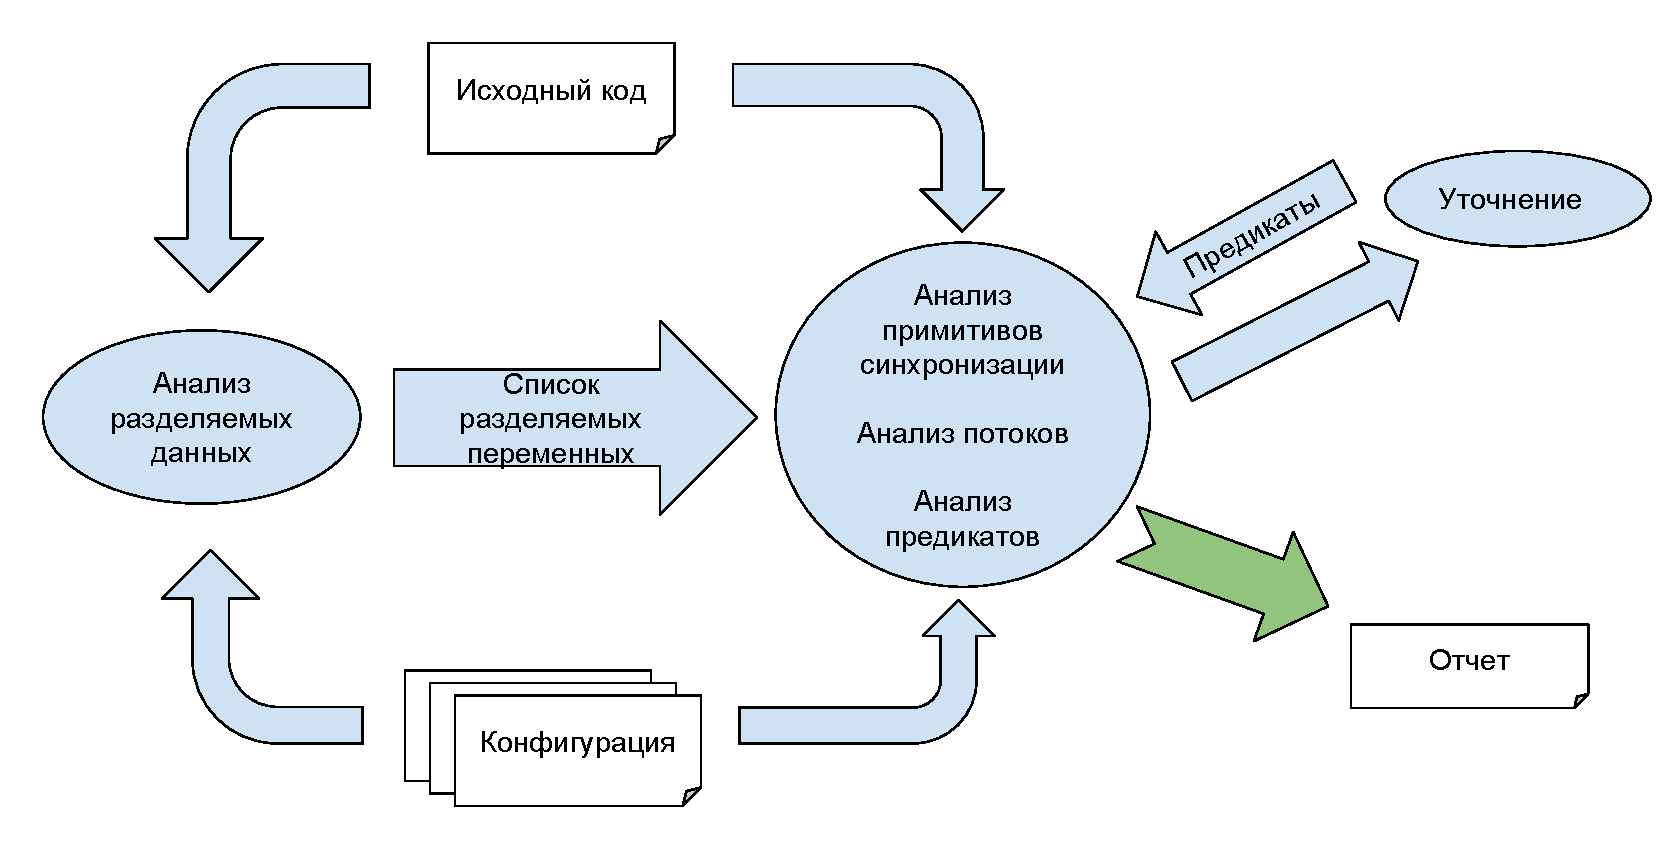
\includegraphics [scale=0.6] {MethodScheme}
  \caption{Общая схема метода}
  \label{img:method}
\end{figure}

Анализ разделяемых данных состоит из следующих CPA: BAMCPA, CompositeCPA, LocationCPA, CallstackCPA, ThreadCPA, LocalCPA.
\begin{itemize}
\item BAMCPA. Данный CPA реализует оптимизацию кеширования абстрактных блоков. Анализ будет подробно описан в соответствующем разделе.
\item CompositeCPA. Анализ объединяет в себе несколько анализов, в нашем случае, LocationCPA, CallstackCPA и LocalCPA.
\item LocationCPA. Анализ служит для корректного обхода графа потока управления.
Абстрактным состоянием этого анализа является узел графа потока управления, а переход в следующее состояние возможен только по доступным дугам ГПУ из этого узла.
\item CallstackCPA. Анализ служит для обеспечения контекстной зависимости.
Абстрактным состоянием анализа является стек вызовов функций.
Таким образом, вызов одной и той же функции из разных мест не приведет к получению одинакового абстрактного состояния.
\item LocalCPA. Анализ определяет множество разделяемых переменных для данной точки программы.
Информация о локальности данных распространяется по присваиваниям от точек выделения локальной памяти или взятия адреса локальной переменной.
Если для некоторой переменной не известен ее статус, консервативно считается, что память является разделяемой.
\end{itemize}

Основной анализ состоит из следующих CPA: BAMCPA, UsageCPA, CompositeCPA, LocationCPA, CallstackCPA, LockCPA, PredicateCPA, ThreadCPA.
Анализы BAMCPA, CompositeCPA, LocationCPA и CallstackCPA являются теми же, что и в предыдущем случае.
Подробное описание остальных анализов будет приведено далее.
UsageCPA выполняет некоторые оптимизации, связанные с упрощением доступов к памяти.
Например, заменяет доступ к элементу списка на доступ ко всем списку.

Исходный код программы, подаваемый на вход может быть разбит на несколько файлов, но, тем не менее, этот набор должен компилироваться.
Чтобы избежать сложных конструкций языка Си и упростить код, часто применяется инструмент CIL~\cite{CIL}, который, в том числе, может объединять несколько файлов в один.

Результатом анализа является множество предупреждений.
Каждое предупреждение представляет собой пару доступов к разделяемой памяти с непересекающимся множеством блокировок, при этом хотя бы одна из них является записью.
Для каждого доступа к разделяемой памяти восстанавливается один из путей, который может привести к этому доступу.
Формат выходных данных описан в разделе~\ref{sect_impl_visualization}.

\section{Оптимизации хранения данных} \label{sect_impl_storage}

\subsection{Идентификаторы доступа к памяти} \label{subsect_impl_identifiers}

Как уже было описано, состояние гонки определяется, как ситуация, при которой возможен доступ к памяти одновременно из нескольких потоков. 
При реальном выполнении программы запись в одну и ту же ячейку памяти понятен, но возникает вопрос, что подразумевать под одной памятью при статической верификации.
Основной проблемой становятся указатели, значение которых определяется в процессе анализа.
Как уже отмечалось в обзоре, многие точные инструменты статической верификации, в частости инструменты, реализующие методы ограничиваемой проверки моделей, вообще не распространяют свои подходы на программы с указателями, ограничиваясь только глобальными переменными.
В других инструментах, про которых уже говорилось в при обзоре, применяется анализ синонимов (англ. alias) Андерсена.
В этом случае собираются так называемые may-алиасы для каждой переменной, то есть множество областей памяти (адресов), на которые может указывать данный указатель.

Для нашей задачи поиска состояний гонки в системном программном коде не подходит первый способ, хотя при построении математической модели мы ограничились только глобальными переменными.
Поиск алиасов для каждого из нескольких тысяч указателей является слишком трудоемкой задачей.
В итоге необходимо использовать некоторую разумную эвристику, которая позволит определить одну и ту же область памяти. 

Основой предложенной эвристики стало наблюдение, что обычно с одинаковыми указателями в системном программном обеспечении работают похожим образом.
Так, например, в один и тот же указатель обычно записывают похожие данные, которые защищаются одинаковым способом.
В этом случае не обязательно отслеживать, на какую память конкретно указывает некоторый указатель, если к нему обращаются различными способами, например, с использованием примитивов синхронизации, и без них, то это уже является достаточно подозрительным местом.
При этом встречаются случаи, в которых такая эвристика дает ложные срабатывания. 
Предположим, например, что в некоторую функцию передается некоторый указатель на память, которая может быть как локальной, так и разделяемой. 
В этой функции производится некоторая обработка информации. При этом если память является разделяемой, то до вызова функции производится захват блокировки, а в случае, если память является локальной - то захват блокировки не производится.
В этом случае 

%\subsection{Накопление результатов в процессе анализа} \label{subsect_impl_storage}
%
%Для каждого доступа к переменной формируется специальная структура данных, содержащая информацию об этом доступе. 
%Будем использовать обозначение $Usage$ для этой структуры данных.
%
%\begin{align}
%& Usage = (line, access, state, states, id) \nonumber \\ 
%& line \in \mathbb{N}, access \in \{READ, WRITE\}, state \in E, states \in 2^E, id \in ID \nonumber
%\end{align}
%
%Здесь $line$ - номер строки исходного кода, $access$ - тип доступа, $state$ - соответствующее абстрактное состояние из анализа, которое используется для восстановления пути, $states$ - множество состояний различных анализов, которые должны учитываться при определении состояния гонки, $id$ идентификатор переменной, описанный в подразделе~\ref{subsect_impl_identifiers}.
%Множество всех $Usage$ обозначим, как $UsageSet$. 
%Стоит заметить, что множество $states$ извлекается из общего состояния $state$, но какие именно его части важны, определяется тем анализом, который соответствует этому состоянию.
%Например, номер строки исходного кода, который, в числе прочих, является частью состояния LocationCPA, но не является существенной информацией для определения состояний гонки. 
%Состояния LockCPA, содержащих множество захваченных блокировок, используются в алгоритме Lockset для определения потенциальных состояний гонки, поэтому состояния этого анализа присутствуют во множестве $states$. 
%Так, в текущей конфигурации используется информация из состояний ThreadCPA и LockCPA. 
%Для оптимизации сохраняются не полные состояния анализа, а некоторые усеченные варианты, содержащие только необходимую информацию.
%Опять же, какой вариант состояния требуется сохранить для вычисления состояния гонки, определяется сам анализ.
%
%Основной задачей для сохранения результатов в процессе анализа является не обеспечение быстрого доступа и быстрого поиска, а удобство применения оптимизации BAM. 
%Для решения этой задачи была разработана многоуровневая система контейнеров. 
%Как только встречается доступ в разделяемую переменную, формируется $Usage$, который добавляется в небольшой контейнер, связанный с абстрактым состоянием. Обозначим, этот контейнер, как $StateContainer \subseteq UsageSet$.
%Так, при появлении нового $Usage$: $StateContainer := StateContainer \cup Usage$.
%
%В том состоянии, которое соответствует абстрактному состоянию предикатного анализа, все $Usage$ из временного контейнера переносятся в следующий контейнер, соответствующий абстрактному блоку. Обозначим этот контейнер, как $FunctionContainer \subseteq UsageSet$.
%Так, при обновлении контейнера: $FunctionContainer := FunctionContainer \cup StateContainer$.
%Обновление $FunctionContainer$ происходит, только если соответствующее состояние предикатного анализа не является тождественным false.
%Это сделано для того, чтобы исключить из анализа те доступы к переменным, которые расположены на недостижимых путях.
%В случае, если в запуске не используется предикатный анализ, обновление $FunctionContainer$ производится для каждого состояния.
%
%При выходе из абстрактного блока выполняется операция expand для получившегося состояния, в том числе и для $FunctionContainer$.
%Операция expand для контейнера заключается в применении операции expand для каждого элемента $Usage$.
%$expand(FunctionContainer) = \{Usage'=(line, access, state, states', id) \mid \exists Usage=(line, access, state, states, id) \in FunctionContainer \land states'=\{s' \mid s' = expand(s) \land s \in states\} \}$
%После применения операции expand ко всему множеству $Usage$, полученное множество $Usage$ добавляется в контейнер внешнего абстрактного блока.
%Таким образом, информация о всех $Usage$ собирается снизу вверх по графу вызовов до самого main. 
%Одной из проблем являются бесконечные циклы. Если цикл не имеет выхода, это значит, что информация из контейнера, соответствующего этому абстрактному блоку, не будет добавлена в контейнер, соответствующий функции main.
%
%После завершения анализа, то есть при выходе из самого последнего (верхнего) абстрактного блока, информация из соответствующего контейнера добавляется в глобальный контейнер.

\subsection{Устройство глобального контейнера} \label{subsect_impl_global_storage}

После построения абстракции необходимо проверить наличие состояний гонки.
Для этого множество достижимых состояний обходится и вычисляются все возможные доступы к разделяемым переменным.
Необходимо отметить, что обход множества достижимых состояний происходит с учетом оптимизации BAM, которая разбивает это множество на абстрактные блоки в процессе анализа.
Так, один и тот же абстрактный блок может быть достижим при различных характеристиках, например, множестве захваченных блокировок. 
В процессе анализа этот блок анализировался только один раз, так как такая характеристика не влияет на достижимость других состояний, однако, при вычислении возможных состояний гонки информация о захваченных блокировках становится важной.


Для каждого доступа к переменной формируется специальная структура данных, содержащая информацию об этом доступе. 
Будем использовать обозначение $Usage$ для этой структуры данных.

\begin{align}
& Usage = (line, access, state, states, id) \nonumber \\ 
& line \in \mathbb{N}, access \in \{READ, WRITE\}, state \in E, states \in 2^E, id \in ID \nonumber
\end{align}

Здесь $line$ - номер строки исходного кода, $access$ - тип доступа, $state$ - соответствующее абстрактное состояние из анализа, которое используется для восстановления пути, $states$ - множество состояний различных анализов, которые должны учитываться при определении состояния гонки, $id$ идентификатор переменной, описанный в подразделе~\ref{subsect_impl_identifiers}.
Множество всех $Usage$ обозначим, как $UsageSet$. 
Стоит заметить, что множество $states$ извлекается из общего состояния $state$, но какие именно его части важны, определяется тем анализом, который соответствует этому состоянию.
Например, номер строки исходного кода, который, в числе прочих, является частью состояния LocationCPA, но не является существенной информацией для определения состояний гонки. 
Состояния LockCPA, содержащих множество захваченных блокировок, используются в алгоритме Lockset для определения потенциальных состояний гонки, поэтому состояния этого анализа присутствуют во множестве $states$. 
Так, в текущей конфигурации используется информация из состояний ThreadCPA и LockCPA. 
Для оптимизации сохраняются не полные состояния анализа, а некоторые усеченные варианты, содержащие только необходимую информацию.
Опять же, какой вариант состояния требуется сохранить для вычисления состояния гонки, определяется сам анализ.

Задачей глобального контейнера является обеспечение быстрого поиска состояний гонки среди всех добавленных состояний. 
На верхнем уровне контейнер содержит отображение из идентификатора переменной в специальное множество, содержащее $Point$.
$Point$ - это срез информации, содержащейся в $Usage$, которая может повлиять на наличие состояние гонки.
Множество всех $Point$ обозначим через $PointSet$.

\begin{align}
& Point = (access, states, covered) \nonumber \\ 
& access \in \{READ, WRITE\}, states \in 2^E, covered \in PointSet \nonumber
\end{align}

При построении $Point$ необходимая информация извлекается из $Usage$: $Usage = (line, access, state, states, id) \implies point(Usage) = (access, states, \emptyset)$.
Множество $covered$ - это множество покрытых $Point$: $Point = (access, states, covered) \land Point \neq Point'=(access', states', covered') \in covered \Leftrightarrow \forall e' \in states' \exists e \in states: e' \sqsubseteq e \land (access' = access \lor access' = READ)$.
Одно из важных свойств $race(point_1, point_2) \land point_2 \in covered(point_3) \implies race(point_1, point_3)$.
Таким образом можно сократить перебор при поиске состояния гонки. 
Например, если имеется доступ к одной переменной с пустым множеством блокировок и с захваченной блокировкой, в первую очередь необходимо рассмотреть доступ, который производится без блокировок.

Глобальный контейнер хранит для каждого идентификатора множество $Point$, которые ему соответствуют, и отдельно множество $topSet \subseteq PointSet$, тех $Point$, которые не покрываются никакими другими $Point$.
$GlobalContainer = \{id \mapsto P\}, id \in ID, P = (topSet, pMap), pMap = \{Point \mapsto uSet\}, uSet \subseteq UsageSet$.
Обозначим $points(id) = \bigcup_{pMap \in GlobalContainer(id)}{dom(pMap)}$ - множество всех $Point$, соответствующих одному идентификатору, которые были получены в процессе анализа.
$usages(id) = \bigcup_{Point \in points(id)}{pMap(Point)}$ - множество всех доступов к переменной, которые были получены в процессе анализа.

Проверка наличия состояния гонки сводится к перебору $Point \in topSet$, размер которого значительно меньше, чем размер исходного $UsageSet$.
Покажем, что такая оптимизация корректна, то есть, 
$\exists usage_1, usage_2 \in usages(id): race(usage_1, usage_2) \Leftrightarrow \exists point_1, point_2 \in topSet: race(point_1, point_2)$.
$race(usage_1, usage_2) = \forall s \in states_1 \exists s' \in states_2: compatible(s, s') \land (access_1 = WRITE \lor access_2 = WRITE)$.
Если $point_1=point(usage_1) \land point_2=point(usage_2)$ доказательство очевидно, так как множества $states$ у них одинаковые.
Рассмотрим случай $point_1 =point(usage_1) \land point(usage_2) = point' \in covered(point_2)$. 
Покажем, что $race(point_1, point') \implies race(point_1, point_2)$, то есть мы не пропустим состояние гонки, рассмотрев только множество $topSet$. 
$race(point_1, point') = \forall s \in states_1 \exists s' \in states': compatible(s, s') \land (access_1 = WRITE \lor access' = WRITE)$.
Так как $\forall s, s_1, s_2 \in E: s_1 \sqsubseteq s_2 \land compatible(s, s_1) \implies compatible(s, s_2)$, получаем $\forall s \in states_1 \exists s' \in states_2: compatible(s, s')$.
$(access_1 = WRITE \lor access' = WRITE) \land (access' = access_2 \lor access' = READ) \implies (access_1 = WRITE \lor access_2 = WRITE)$.
Оба условия выполнены, поэтому будет найдено состояние гонки на множестве $topSet$. 

Нужно отметить, что в данном случае нас не интересует истинность найденных состояний гонки.
Подробно процесс уточнения будет представлен в подразделе~\ref{sect_impl_refinement}.
Процесс уточнения позволяет исключить из абстракции локально-недостижимые пути, а также состояния гонки, ошибочно найденные из-за неточностей других анализов.
Однако, для того, чтобы исключить все локально-недостижимые пути может потребоваться большое количество уточнений и перестроений абстракции.
Чтобы не проверять каждый раз те пути, для которых доказана их достижимость, нужно каким-то образом сохранять информацию об уже проведенных уточнениях.

Как было описано выше, имеется два уровня абстракции над всем множеством доступов к переменной:
множество доступов к одной и той же переменной (множество $Usage$), и множество доступов к одной переменной с одними и теми же параметрами (множество $Point$).
Для того чтобы получить истинное состояние гонки для одной переменной, нам необходимо получить два истинных пути, ведущих к этой переменной. 
Если для некоторой переменной были найдены такие пути, которые образуют состояние гонки, значит, больше нет необходимости собирать информацию для этой переменной. Эта переменная помечается специальным образом и больше не участвует в уточнении.

\subsection{Пример представления данных} \label{subsect_impl_example}

Рассмотрим такой фрагмент исходного кода.

\begin{verbatim}
int global;
...
int dummy_function(){
  int local;
  ...
  global = 1;
  mutex_lock(&mutex);
  local = global;
  mutex_unlock(&mutex);
  ...
  mutex_lock(&mutex);
  local = local + global;
  mutex_unlock(&mutex);
}
\end{verbatim}

Часть $GlobalContainer$ для этого фрагмента программы представлена на рисунке~\ref{img:globalcontainer}. 

\begin{figure}[ht] 
  \centering
  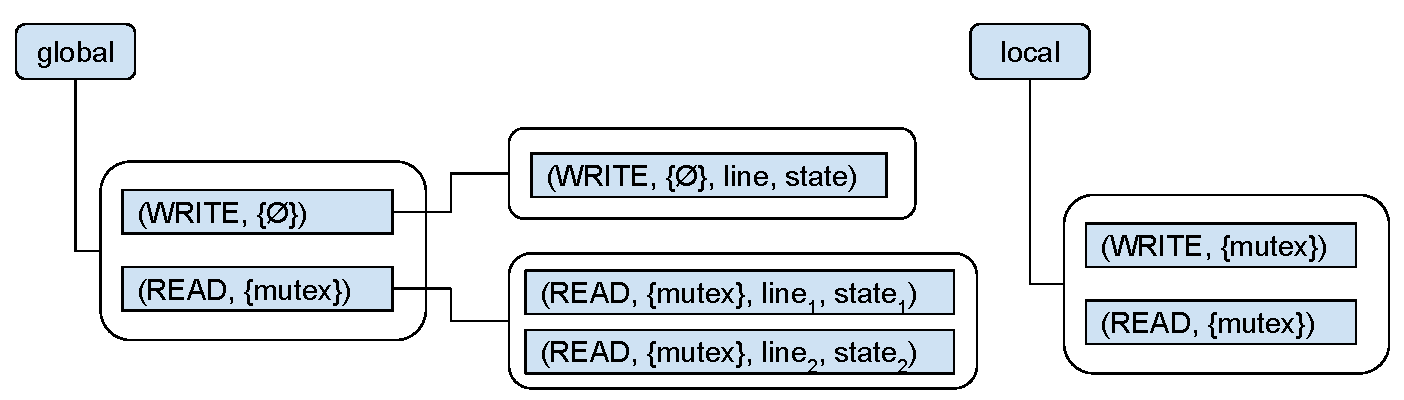
\includegraphics [scale=0.7] {GlobalContainer}
  \caption{Пример}
  \label{img:globalcontainer}
\end{figure}

Переменной $global$ соответствуют две точки использования: запись без использования примитивов синхронизации и чтение при захваченной mutex-блокировке. 
Причем второй точке использования соответствуют два реальных доступа, расположенных в разных строках исходного кода.

\section{Реализация уточнения} \label{sect_impl_refinement}

Уточнение абстракции по контрпримерам используется для того, чтобы исключить недостижимые пути из абстракции.
В классическом варианте CEGAR используется при решении задачи достижимости.
Когда найдено ошибочное состояние, начинается процесс уточнения: строится контрпример и проверяется, возможен ли такой сценарий в исходной программе. В случае, если такой путь является недостижимым из-за неточности абстракции, она уточняется таким образом, чтобы исключить такой путь из абстракции. 

При поиске состояний гонки дело усложняется тем, что ошибкой является не одно состояние, а пара. При этом каждый из путей сам по себе не является ошибкой.
Кроме того, обычно требуется обнаружить не первое состояние гонки в программе, а все потенциальные состояния гонки. 
Таким образом, возможны две вариации процедуры уточнения абстракции.

\begin{enumerate}
\item Уточнение производится в процессе анализа. При обнаружении пары состояний, составляющих состояние гонки, оба пути проверяются на достижимость. Если найденная ошибка подтверждается, она отмечается, как подтвержденная и анализ продолжается.
Этот вариант уточнения очень похож на классический вариант: при обнаружении ошибки абстракция уточняется до тех пор, пока ошибка либо не подтвердится, либо не опровергнется.
Такой подход обладает существенным недостатком: для корректного завершения анализа, требуется построить очень точную абстракцию. 
В случае, если анализируемый код содержит сотни тысяч строк кода, построение точной абстракции требует колоссального времени. 
Более эффективно в этом случае гибко задавать ограничения на ресурсы, чтобы иметь возможность завершить анализ в любой момент, хотя это и повлечет за собой некоторое снижение точности. 
Это позволяет сделать второй подход к уточнению.

\item Уточнение всех путей производится в тот момент, когда абстракция полностью построена. Все обнаруженные состояния гонки проверяются на истинность, и, в случае необходимости, абстракция перестраивается. 
Существенным недостатком этого подхода является большой объем лишней работы в том случае, если неточность абстракции затрагивает множество состояний гонки.
Тогда проверка каждой из них будет давать один и тот же результат.
Однако, возможно применение некоторых оптимизаций, которые позволяют сократить время на такую бесполезную работу. 
\end{enumerate}

Нужно отметить, что оба варианта уточнения способны исключать из абстракции только локально-недостижимые пути.
Пути, в которых неправильно моделируется взаимодействие потоков, не могут быть исключены из абстракции.

Для того, чтобы обеспечить гибкую настройку, процесс уточнения был разделен на функциональные блоки.
Каждый такой блок определяется тем, что он принимает себе на вход от предыдущего блока, и тем, что он выдает на выходе следующему.
Результатом работы каждого из абстрактных блоков является вердикт TRUE, означающий, что то, что передается на вход этому блоку, содержит состояния гонки, и вердикт FALSE, означающий, что состояние гонки обнаружить не удалось.
В последнем случае может быть выдана некоторая информация (precision), которая позволит более точно вычислить абстракцию на следующей итерации анализа.
В редких случаях возможен вердикт UNKNOWN, означающий, что однозначный ответ не может быть получен. 
В большинстве случаев такой вариант реализуется при некорректной работе сторонних компонентов, таких как решателей (англ. solver).

Цепочка блоков уточнения состоит из двух частей. Первая часть - служебная, которая используется для подготовки путей к уточнению и обработке полученной от других блоков информации. Эта часть содержит:

\begin{enumerate}

\item IdentifierIterator. Блок, принимающий на вход ReachedSet и последовательно перебирающий все возможные переменные, к которым был доступ.
Соответственно, следующий за ним блок обязан принимать на вход идентификатор переменной.
В случае, если хотя бы для одной переменной был получен вердикт FALSE, это означает, что уточнение прошло успешно, и необходимо перестроить абстракцию.
Если же для всех новых переменных вердикт был TRUE или UNKNOWN, это означает, что абстракция построена с достаточным уровнем точности, и все найденные состояния гонки являются истинными с точки зрения анализа.

Каждый вердикт FALSE сопровождается некоторой информацией о том, как следует уточнить абстракцию. Этот уровень точности сохраняется для каждой переменной отдельно, но при построении абстракции учитывается уровень точности, полученный для каждой из переменных. Однако, в случае если для  какой-либо переменной будет доказано, что она участвует в истинном состоянии гонки, то соответствующий этой переменной уровень точности сбрасывается. Это помогает не перестраивать слишком точную абстракцию тогда, когда это уже не нужно.

\item PointIterator. Блок, принимающий на вход идентификатор переменной и перебирающий все возможные пары $Point$, которые образуют состояние гонки. Каждая пара $Point$ проверяется следующим блоком. Если для некоторой пары $Point$ будет получен вердикт TRUE, это означает, что ни один следующий блок не смог найти противоречия, а значит, полученное состояние гонки истинное и в предыдущий блок возвращается результат TRUE. 

\item UsageIterator. Блок, принимающий на вход пару $Point$ и перебирающий все возможные пары $Usage$, соответствующие этой паре $Point$. Каждая пара $Usage$ проверяется следующим блоком. Если для некоторой пары $Usage$ будет получен вердикт TRUE, это означает, что ни один следующий блок не смог найти противоречия, а значит, полученное состояние гонки истинное и в предыдущий блок возвращается результат TRUE. 

\item PathIterator. Блок, принимающий на вход пару $Usage$ и перебирающий все возможные пары путей в абстракции, соответствующие этой паре $Usage$. Необходимо пояснить, почему в абстракции возможно несколько путей из начального состояния к тому состоянию, которое соответствует данному $Usage$. Дело в том, что из-за применении оптимизации BAM (подраздел~\ref{subsect_impl_bam}), тело функции будет проанализировано один раз, несмотря на то, что вызовов этой функции может быть несколько. В таких случаях для каждого вызова функции возможно несколько точек ее вызова. Если для некоторой пары путей будет получен вердикт TRUE, это означает, что ни один следующий блок не смог найти противоречия, а значит, полученное состояние гонки истинное и в предыдущий блок возвращается результат TRUE. 

\end{enumerate}

Далее идет вторая часть цепочки, которая занимается непосредственно проверкой корректности двух путей. Поэтому каждый из этих блоков принимает на вход и передает в следующий блок пару путей. Если текущий блок считает, что данная пара путей невозможна, в предыдущий блок возвращается результат FALSE.
Блоки уточнения из этой части не являются обязательными, поэтому допустима любая их комбинация.

\begin{enumerate}

\item PredicateRefiner. Основной инструмент для удаления из абстракции локально-недостижимых путей. 
Использует внутри себя классический PredicateRefiner, но дополнительно применяется некоторый набор оптимизаций для того, чтобы сократить время работы.
Например, при переборе всех возможных пар путей может часто возникать проверка отдельного пути на локальную-достижимость. 
Чтобы избежать лишних проверок, сохраняется результат каждого уточнения для пути, а также тот уровень точности, который нужен для исключения данного пути из абстракции.
Таким образом, если возникнет необходимость в уточнении этого же пути, не важно на этой же итерации уточнения или на любой из последующих, выдет использован сохраненный результат. 

\item Фильтр. Фильтром называется такой блок, который, выдавая результат FALSE, не предоставляет уровень точности для того, чтобы исключить полученный путь (пару путей) из абстракции. А это значит, что такая же пара путей будет получена и для следующей абстракции.
Такой фильтр, тем не менее, полезен тем, что при переборе всех подходящих путей может быть найдена такая пара, которая будет истинна.
Возможны различные варианты фильтров, например, такой, который отсеивает доступы к переменным, происходящим из специальных функций. 

\end{enumerate}

Последний блок в цепи является специальной заглушкой, которая всегда возвращает значение TRUE.

Оптимизированный вариант?

\section{Печать и визуализация} \label{sect_impl_visualization}

Визуализация найденных состояний гонок является важным моментом для практического применения инструмента.
Выдаваемой информации должно быть достаточно для того, чтобы разработчик смог понять, какие именно действия в программе могут привести к состоянию гонки.
Таким образом, основными требованиями к визуализации являются:

\begin{enumerate}

\item Отображение всех операторов, которые встречаются на пути к каждому из доступов, образующих состояние гонки

\item Отображение и визуальное выделение двух доступов, образующих состояние гонки

\item Отображение и визуальное выделение всех операций с примитивами синхронизации

\item Отображение справочной информации о состоянии гонки: множество захваченных примитивов синхронизации, тип и имя разделяемой переменной

\end{enumerate}

Основой формата вывода найденных состояний гонки является формат, описанный в .
Этот формат предполагает преставление пути к ошибке в виде графа, который содержит одну исходную вершину, вершину, которая соответствует нарушению спецификации и некоторое множество промежуточных вершин.
Ребра графа соответствуют дугам графа потока управления.

Граф пути обычно имеет линейную структуру, хотя формат позволяет описывать различные ветвления, например, циклы, которые удобнее визуализировать, не разворачивая все выполненные итерации.
Так как разработанный инструмент реализцет метод с раздельным рассмотрением потоков, то мы не может однозначно указать порядок выполнения инструкций (чередование потоков).
Поэтому все инструкции каждого потока идут последовательно друг за другом, то есть, сначала начинается главный поток, который выполняется до точки, в которой происходит разделение путей, ведущих к двум доступам к памяти.
Обычно, это происходит при создании некоторого потока.
После этого продолжается первый путь, который приводит к первому доступу к памяти.
Далее отображаются операторы второго пути, начинающиеся с той точки разветвления.
Таким образом для пользователя будет выведено сначала трасса, ведущая к первому доступу, а затем, трасса ко второму доступу.

Пример визуализированной трассы представлен на рисунке~\ref{img:error_trace}.

\begin{figure}[ht] 
  \centering
  \includegraphics [scale=0.5] {ErrorTraceExample}
  \caption{Пример визуализированного предупреждения}
  \label{img:error_trace}
\end{figure}

%\newpage
%============================================================================================================================

\clearpage